\chapter{Background estimate}
\label{ch:bkg}
\epigraph{\emph{“Champions keep playing until they get it right.”}}{Billie Jean King}




With the event selection described in \Ch{\ref{ch:evt_selection}}, events with fragmentation photons and \(t\)-channel events were highly reduced and the signal significance was increased as well, providing an excellent scenario for bump searches. Now, in this chapter in \Sect{\ref{sec:bkg:estimation}}, the background estimation in these signal regions is described, in particular the ones from where a jet fakes a photon. The background in this type of resonance search is modeled with an analytical function, and several statistical tests are needed in order to define it. In \Sect{\ref{sec:bkg:modeling}}, the selection of the optimal function(s) is presented, where all the statistical tests to achieve so are discussed in detail.




\section{Background estimation: jet faking photons}
\label{sec:bkg:estimation}

It was discussed in \Ch{\ref{ch:strategy}} that the main backgrounds encountered for this analysis are those in which there is at least a photon and a jet in the final state. Although \ac{SM} \gammajet events (prompt photons discussed in \Sect{\ref{subsec:theory:sm:prompt_photon}}) is the dominant background, jet faking photons events is another important source of background that need to be taken into account.

% Emphasizing again, backgrounds in this analysis are only estimated to optimise the modeling of it, that is, finding the most optimal function that can describe it, henceforth, not involving them in the final calculations with data. \fixme{add this?}


Jets can be misidentified as photons (fake photons) if they fluctuate to \pizero's (in a dominant way), resulting in an \ac{EM} object indistinguishable from a single, real, highly energetic photon (also called prompt photon). To cope with the large jet backgrounds, the \texttt{Tight} identification criteria is applied on photon candidates. This selection is expected to contain prompt photons with moderate jet contamination. As this misidentification rate is not expected to be accurately modeled in \ac{MC}, a data-driven determination has been used. The \texttt{Tight} offline identification is by design tighter than the photon trigger used to collect the data, so there are quite a few photon candidates from jets that will fail the \texttt{Tight} \ac{WP} but satisfy some intermediate selection. These photon-like jets, from hereinafter called pseudo-photons (or \texttt{Non-Tight}), are defined as those passing the \texttt{Loose} identification but failing (at least) one of \wone, \fside, \deltae, \eratio \texttt{Tight} selection cuts \cite{ATLAS-EGamma-Performance-2015-2017}.

To estimate the number of jet faking photons in the signal regions of the present analysis a combination of two methods is employed. Using the so-called ABCD method with the different expected isolation profiles for both real and fake photons, it is possible to estimate fake factors that allow the calculation of the fakes in signal regions~\cite{ATLAS-SUSY-PhotonMetX-13TeV,ATLAS-SUSY-PhotonMetX-13TeV-NOTE,ATLAS-SUSY-PhotonJetMet-13TeV,ATLAS-SUSY-PhotonJetMet-13TeV-NOTE}. The second method, by making use of a sequential template-fit procedure to the photon isolation distribution in data and \ac{MC}, allows to correctly count the number of real and fake photons in the regions delimited by the ABCD method.

\begin{table}[ht!]
    \centering
    \caption{Baseline event selection used for the jet fakes estimation using the template fit procedure. \ptiso is defined as shown in \Eqn{\ref{eq:objects:egamma:iso:definitions}}.\fixme{revise selection on jet pt}}
    \begin{tabular}{| l | c |}
        \hline
                                        & Selection \\ \hline
        Trigger                         & HLT\_g140\_loose \\ \hline
        \ngamma                         & \(\ge1\) \\ \hline
        \ptgam [GeV]                    & \(>150\) \\ \hline
        \ptjet [GeV]                    & \(> 60\) \\ \hline
        \njets                          & \(>0\) \\ \hline
        \nlep                           & \(0\) \\ \hline
        Track isolation                 & \(\ptiso < 0.05\) \\ \hline
        \(|\etagam|\) acceptance region & \etagamacc \\ \hline
        \myj [GeV]                      & \(\myj > 500\) \\ \hline
    \end{tabular}
    \label{tab:bkg:estimation:selection}
\end{table}

The study uses \texttt{Loose} identification and non-isolated photons and the event selection taking part in this study is shown in \Tab{\ref{tab:bkg:estimation:selection}}.
It is important to notice that the \texttt{Tight} and isolated photons used in the search are only a sub-set of those used in this background-estimation study. By requiring the \texttt{Loose}, non-isolated, photons to pass the selection shown in \Tab{\ref{tab:bkg:estimation:selection}}, \texttt{Tight} identification and \(\etiso < 0 ~\gev\) (see \Eqn{\ref{eq:objects:egamma:iso:definitions}}), one recovers the \texttt{Tight} and isolated photons used in the search.
Finally, a manual Overlap-Removal procedure is carried out between the photons and jets, to remove jet overlapping with the leading \texttt{Loose} photon if \(\dryj<0.4\).
This method, as previously mentioned, is data-driven. Given that unblinding of the full Run-2 data is not performed up to the last analysis stage, only the 2015+2016 dataset is used, as it was already unblinded in a previous work by the \ac{ATLAS} collaboration~\cite{ATLAS-PhotonJetResonances-2016}.


\subsection{ABCD method}
\label{subsec:bkg:estimation:abcd}

The ABCD method defines a signal region \(A\) and three control regions, namely \(B\), \(C\) and \(D\).
These regions are defined by varying the identification status between \texttt{Tight} and \texttt{Non-Tight}, and also by changing the calorimetric isolation requirements (isolated and non-isolated)~\cite{ATLAS-EXOTICS-Monophoton-2017}.
The complete definition of the ABCD regions is given as:
\begin{itemize}
    \item Region \(A\): \texttt{Tight} photons and \(-20 < \etiso < 0~ \gev\)
    \item Region \(B\): \texttt{Tight} photons and \(8 < \etiso < 80~ \gev\)
    \item Region \(C\): \texttt{Non-Tight} photons and \(-20 < \etiso < 0~ \gev\)
    \item Region \(D\): \texttt{Non-Tight} photon and \(8 < \etiso < 80~ \gev\)
\end{itemize}
where \etiso was defined in \Eqn{\ref{eq:objects:egamma:iso:definitions}}. \Fig{\ref{fig:bkg:estimation:abcd:diagram}} shows the resulting four different regions.

\begin{figure*}[ht!]
    \centering
    \includegraphics[width=0.65\textwidth]{5_resonances/bkg/estimation/ABCD_data_regions}
    \caption{Identification vs. \(\etiso\) two-dimensional distribution from data events for the Full Run-2 dataset.}
    \label{fig:bkg:estimation:abcd:diagram}
\end{figure*}

Assuming that there is no signal contamination in any control region, the \(B\), \(C\) and \(D\) regions are only composed of background \(N_{(B,C,D)}=N^{b}_{(B,C,D)}\). In addition assuming no correlation between isolation and the considered shape variables, the following relation holds: \(N^{b}_{B}/N^{b}_{A}=N^{b}_{D}/N^{b}_{C}\). Moreover, two different \acp{FaF} could be defined:
\begin{equation*}
    \ffiso = \frac{N_{C}}{N_{D}} \qquad \ffid = \frac{N_{B}}{N_{D}}
\end{equation*}
Therefore, the number of jets faking photons can be estimated using the \ac{FaF} as:
\begin{equation}
    \label{eq:bkg:estimation:abcd:njfakes}
    N_{\jfake} = N_{A} = \ffiso \times N_{B}  = \ffid \times N_{C}.
\end{equation}

So two different approaches could be used: to model the fake photons using the \texttt{Tight} but non isolated photons from region \(B\) using \ffiso or model the fake photons using the \texttt{Non-Tight} but isolated photons using the \ffid.
Even though both approaches give equivalent results, the \ffiso approach is used as it leads to higher statistics.
%the systematic uncertainties are found to be lower.

Using the \ac{FaF}, now it is possible to estimate the jet-faking photons background contribution in each region of the analysis (\(R\)). To this end, a jet control region (CRJ-R) is defined equally to the region \(R\) but replacing the isolation requirements with the one used in region \(B\), and weighted by the corresponding \ffiso:
\begin{equation*}
    N^{R}_{\jfake}(\pt) = \ffiso(\pt)\cdot N_{\text{CRJ-R}}(\pt)
\end{equation*}





\subsection{Corrections to the ABCD method}
\label{subsec:bkg:estimation:abcd_corrections}

Several corrections can be applied to the ABCD method.
The first one is to consider the possibility of a signal contamination in any of the control regions \(B\), \(C\) or \(D\). By subtracting the amount of signal events in these regions, \Eqn{\ref{eq:bkg:estimation:abcd:njfakes}} becomes:
\begin{equation}
    \label{eq:bkg:estimation:abcd_corrections:njfakes_leak}
    N_{\jfake} = \frac{N_{B} - N_{B}^{s}}{N_{D} - N_{D}^{s}} \times (N_{C} - N_{C}^{s})
\end{equation}
where \(N_{(B,C,D)}^{s}\) is the number of real photons in each region. The estimation of these numbers is a complicated task, since it is needed to have a correct description of the real photons in data, and it is highly contaminated with fake photons. The calculation of the number of real photons in data is performed with an iterative template fit method to the calorimetric isolation distribution in data, explained in more detail below.


The presence of a residual correlation of the background across the four regions, which may manifest itself as a difference in the background distributions for the \texttt{Tight} and \texttt{Non-Tight} regions could be taken into account by calculating:
\begin{equation*}
    R = \frac{N^{b}_{A}\,N^{b}_{D}}{N^{b}_{B}\,N^{b}_{C}} \neq 1.
\end{equation*}

However, since \(R\) can not be found in data because that would mean to obtain \(N_A\), an equivalent parameter is calculated, which can also be written using real photons (leakage photons) subtraction:

\begin{equation*}
    R' = \frac{N_{A'}\,N_{D'}}{N_{B'}\,N_{C'}} = \frac{(N_{A'} - N^{s}_{A'})\,(N_{D'}-N^s_{D'})}{(N_{B'}-N^s_{B'})\,(N_{C'}-N^s_{C'})}
\end{equation*}
with the definition for each primed region being:
\begin{itemize}
    \item region \(A'\): \texttt{Tight} photons and \(8 < \etiso < 15~ \gev\).
    \item region \(B'\): \texttt{Tight} photons and \(16 < \etiso < 80~ \gev\).
    \item region \(C'\): \texttt{Non-Tight} photons and \(8 < \etiso < 15~ \gev\).
    \item region \(D'\): \texttt{Non-Tight} photons and \(16 < \etiso < 80~ \gev\).
\end{itemize}


The particular selection of 8 \gev\ aims to define a background only region, but keeping enough statistics to compute the \(R'\) values. In \Fig{\ref{fig:bkg:estimation:abcd_corrections:rprime}} the \(R'\) values are shown as a function of \ptgam.
The values are very close to 1 with some exceptions in which the values deviate from 1 by a maximum amount of \(\approx 20\%\) at low \ptgam.
\begin{figure}[htbp]
    \centering
    \includegraphics[width=0.5\linewidth]{5_resonances/bkg/estimation/coefficients/can__R__lpidNom__lph_pt0__abslph_etas20_0__2015_2016}
    \caption{\(R'\) values computed as a function of \ptgam. The error bars shown correspond to the statistical uncertainties.}
    \label{fig:bkg:estimation:abcd_corrections:rprime}
\end{figure}



Finally, taking into account the leakage and possible correlations, the \Eqn{\ref{eq:bkg:estimation:abcd_corrections:njfakes_leak}} for the expected number of jet fakes results:
\begin{equation}
    \label{eq:bkg:estimation:abcd_corrections_ffiso}
    N_{\jfake}(\pt) =
    N^{b}_{A} =
    \left[R'  \frac{N_{C}-N^{s}_{C}}{N_{D}-N^{s}_{D}}  \left(1 - \frac{N^{s}_{B}}{N_{B}} \right)\right] \times N_B = \ffiso(\pt)  \times  N_{B}(\pt).
\end{equation}

% In case of working with \ffiso, the systematic uncertainties are evaluated by varying the definition of the \texttt{Non-Tight} objects, namely the \textit{tight-3} (failing at least one of \(w_{s3}\), \fside, \deltae) and \textit{tight-5} (failing at least one of \(w_{s3}\), \fside, \deltae, \eratio and \wstot). On the other hand, for \ffid, systematic variations correspond to change the gap set between regions \(A\) and \(C\) with \(B\) and \(D\). In the nominal case the gap is of \(8~\gev\) and the variations correspond to gaps of 5 and \(11~\gev\). As another systematic variation, for both types of fake factors, to account for the differences introduced by the residual correlation between regions, \(R'\) is set to 1, and it is also calculated using the number of fake photons (instead of data with signal leakage).




\subsection{Template fits procedure}
\label{subsec:bkg:estimation:fits}


In order to estimate the number of jet faking photons in the signal regions of the analysis, it is necessary to have an estimate on the number of events with real photons in the ABCD control regions \(B\), \(C\) and \(D\). To achieve this, a series of fits to the data and real-photon \ac{MC} photon isolation distribution is carried out for both \texttt{Tight} and \texttt{Non-Tight} photons. The final objective of the iterative fits, is to have real- and fake-photon components fits to the data distribution, that will then be used to compute the number of real photons in the ABCD control regions. The procedure uses the \ac{MC} \pythia samples, which are expected to be real photons, hence the leak photon contribution will be very small. The calculation is performed in 11 \ptgam bins:
\[
    \ptgam: \left[ 150, 200, 250, 300, 350, 400, 450, 500, 550, 625, 725, 900, \infty \right]~\gev.
\]


The shape of the calorimetric isolation \etiso is fitted in an iterative fashion, using photons passing the \texttt{Tight} and loose-prime \texttt{Non-Tight} identification criteria, as explained above. 
By definition, events with \(\etiso<0~\gev\) pass the calorimetric isolation requirement and correspond to photons falling in region \(A\) if they are \texttt{Tight}, or \(C\) if they are \texttt{Non-Tight}. On the other hand, events with \(\etiso>0~\gev\) define regions \(B\) (\texttt{Tight} photons) and \(D\) (\texttt{Non-Tight} photons).
In what follows, real photons leaked into the \texttt{Non-Tight} regions will referred as leaked photons. Both \texttt{Tight} and \texttt{Non-Tight} photons will contain a fake component, which will dominate over the leaked photons in the latter case~\cite{ATLAS-DiPhotonSearchIsolation-NOTE,ATLAS-EleMuPhoIsolation-NOTE}.

The sequence of fits proceeds as follows:
\begin{enumerate}
    \item \underline{\texttt{Tight} \ac{MC} photons fit}: Given prompt photon samples provides a good description of \texttt{Tight} photons, its \etiso distribution is fitted with a \ac{CBall} function\footnote{This function consists of a Gaussian core but one of the tails of it follows a power-law form. This function was named after the Crystal Ball Collaboration.}. It was found that the simple \ac{CBall} desription does not accomodate well in the whole range, specially in the bulk of the \etiso distribution, therefore a more flexible function is employed. In this way, an improved version of the \ac{CBall} is used, namely the \ac{DSACB} function\footnote{As it names suggests, in the \ac{DSACB} function, the two tails are modeled by power-law functions, and the core of the Gaussian distribution has two different standard deviations, hence the asymmetry.}. Although the description is much better in this case, the Gaussian core struggles to model correctly the peak of the distribution.
    \item \underline{\texttt{Non-Tight} data leak subtraction}: Using the leak photon component from \ac{MC}, the fake photon shape is estimated by subtracting the leak photons histogram to data in the whole \etiso range. This provides a very good description of the fake photon component in the \texttt{Non-Tight} region.
    \item \underline{\texttt{Tight} data composite fit}: Using the real photons \ac{DSACB} shape estimated in the first step and the fake photons shape estimated in the previous step, a composite fit is performed to the \texttt{Tight} photons \etiso distribtution in data. An example of the resulting fit in three different \pt-bins is shown in \Fig{\ref{fig:bkg:estimation:fits_tightID_data}}.

        The final composite distribution is in good agreement with data, indicating the correct selection of the distributions for each component. The real photons component is the responsible for the high peak at low isolation values, while the fake components contributes mainly in the range \(0~\gev < \etiso < 40 ~\gev\), but having a much smaller yield, as expected. Some differences between the model and data can be seen near the peak of the distribution, as indicate by the fit pull. This difference was also seen in the first step of the calculation when modeling the real photon components, and it is directly originating from the gaussian modeling of the real photons peak.

        \begin{figure}[bth!]
            \centering
            \begin{subfigure}[h]{0.32\linewidth}
                \centering
                \includegraphics[width=\linewidth]{5_resonances/bkg/estimation/fits/lpid4/2015_2016/lph_pt0/lph_pt0__250p0/data__tight__composite__lph_pt0__250p0__abslph_etas20__0p00}
                \caption{\(250 < \ptgam < 300~\gev\).}
            \end{subfigure}
            \begin{subfigure}[h]{0.32\linewidth}
                \centering
                \includegraphics[width=\linewidth]{5_resonances/bkg/estimation/fits/lpid4/2015_2016/lph_pt0/lph_pt0__450p0/data__tight__composite__lph_pt0__450p0__abslph_etas20__0p00}
                \caption{\(450 < \ptgam < 500~\gev\).}
            \end{subfigure}
            \begin{subfigure}[h]{0.32\linewidth}
                \centering
                \includegraphics[width=\linewidth]{5_resonances/bkg/estimation/fits/lpid4/2015_2016/lph_pt0/lph_pt0__725p0/data__tight__composite__lph_pt0__725p0__abslph_etas20__0p00}
                \caption{\(725 < \ptgam < 900~\gev\).}
            \end{subfigure}
            \caption{Composite fit to data. The red curve represents the real photons component which is represented by a \ac{DSACB} distribution, computed in the first step. The yellow histogram is the fake photon contribution, obtained via leak-photon subtraction in the previous step. The lower pad of the figures represent the normalised residuals (or pull) of the fits.}
            \label{fig:bkg:estimation:fits_tightID_data}
        \end{figure}
\end{enumerate}





\subsection{Results}
\label{subsec:bkg:estimation:results}

From the above procedure using the ABCD and the template-fit methods, several key figures can be extracted. One important variable, to gain understanding of the phyiscs process, is the \gammajet purity, calculated as:
\[
    P_A = \frac{
        N^{A}_{\text{real}\gamma, \text{postfit}}
    }{
        N^{A}_{\text{real}\gamma, \text{postfit}} + N^{A}_{\text{fake}\gamma, \text{postfit}}
    }.
\]
These purities are shwon in \Fig{\ref{fig:bkg:estimation:results:results:purities}} and their numerical values in \Tab{\ref{tab:bkg:estimation:results:ffiso_purity_values}}. As it can be observed, purities of \(>92\%\) are achieved throughout the whole \ptgam range, indicating that processes containing a real photon and a jet encompass the majority of the sample.The purity measurements are smoothed using a \(3^{\text{rd}}\) order spline, shown with the red line in the figure.

\begin{table}[ht!]
    \caption{Smoothed photon fake factors \ffiso and \gammajet purity as a function of \ptgam.}
    \begin{tabular}{lcc}
        \toprule
        \(p_{T}^{\text{leading} \gamma}\) [GeV] & \(FF_{\text{iso}}\) &  Purity real \(\gamma\) in A \\
        \midrule
        $150-200$    & $0.1873$ & $0.9201$ \\
        $200-250$    & $0.1885$ & $0.9321$ \\
        $250-300$    & $0.1901$ & $0.9418$ \\
        $300-350$    & $0.1918$ & $0.9494$ \\
        $350-400$    & $0.1934$ & $0.9552$ \\
        $400-450$    & $0.1948$ & $0.9593$ \\
        $450-500$    & $0.1956$ & $0.9620$ \\
        $500-550$    & $0.1956$ & $0.9636$ \\
        $550-625$    & $0.1943$ & $0.9642$ \\
        $625-725$    & $0.1891$ & $0.9633$ \\
        $725-900$    & $0.1703$ & $0.9604$ \\
        $900-\infty$ & $0.0835$ & $0.9650$ \\
        \bottomrule
    \end{tabular}
    \label{tab:bkg:estimation:results:ffiso_purity_values}
    \centering
\end{table}
% \begin{table}[ht!]
%     \caption{Smoothed photon fake factors \ffiso and \gammajet purity as a function of \ptgam.}
%     \begin{tabular}{|l|c|c|c|c|}
%         \hline
%         \(p_{T}^{\text{leading} \gamma}\) [GeV] & \(FF_{\text{iso}}\) & Total \(FF_{\text{iso}}\) Unc. & Purity real \(\gamma\) in A & Total \(P_{A}\) Unc. \\
%         \hline
%         \hline
%         $150-200$ & $0.1873$ & $^{+0.0788 (42.10 \%)}_{-0.0719 (38.38 \%)}$ & $0.9201$ & $^{+0.0338 (3.67 \%)}_{-0.0113 (1.23 \%)}$ \\
%         \hline
%         $200-250$ & $0.1885$ & $^{+0.0640 (33.97 \%)}_{-0.0681 (36.14 \%)}$ & $0.9321$ & $^{+0.0252 (2.71 \%)}_{-0.0105 (1.13 \%)}$ \\
%         \hline
%         $250-300$ & $0.1901$ & $^{+0.0517 (27.22 \%)}_{-0.0641 (33.70 \%)}$ & $0.9418$ & $^{+0.0187 (1.99 \%)}_{-0.0101 (1.07 \%)}$ \\
%         \hline
%         $300-350$ & $0.1918$ & $^{+0.0418 (21.79 \%)}_{-0.0598 (31.18 \%)}$ & $0.9494$ & $^{+0.0141 (1.48 \%)}_{-0.0100 (1.06 \%)}$ \\
%         \hline
%         $350-400$ & $0.1934$ & $^{+0.0340 (17.57 \%)}_{-0.0554 (28.64 \%)}$ & $0.9552$ & $^{+0.0112 (1.17 \%)}_{-0.0103 (1.08 \%)}$ \\
%         \hline
%         $400-450$ & $0.1948$ & $^{+0.0281 (14.45 \%)}_{-0.0509 (26.15 \%)}$ & $0.9593$ & $^{+0.0097 (1.01 \%)}_{-0.0109 (1.13 \%)}$ \\
%         \hline
%         $450-500$ & $0.1956$ & $^{+0.0241 (12.30 \%)}_{-0.0465 (23.79 \%)}$ & $0.9620$ & $^{+0.0096 (0.99 \%)}_{-0.0117 (1.22 \%)}$ \\
%         \hline
%         $500-550$ & $0.1956$ & $^{+0.0215 (11.01 \%)}_{-0.0422 (21.58 \%)}$ & $0.9636$ & $^{+0.0105 (1.09 \%)}_{-0.0128 (1.33 \%)}$ \\
%         \hline
%         $550-625$ & $0.1943$ & $^{+0.0203 (10.45 \%)}_{-0.0371 (19.11 \%)}$ & $0.9642$ & $^{+0.0130 (1.34 \%)}_{-0.0146 (1.51 \%)}$ \\
%         \hline
%         $625-725$ & $0.1891$ & $^{+0.0215 (11.37 \%)}_{-0.0309 (16.32 \%)}$ & $0.9633$ & $^{+0.0180 (1.87 \%)}_{-0.0177 (1.84 \%)}$ \\
%         \hline
%         $725-900$ & $0.1703$ & $^{+0.0280 (16.42 \%)}_{-0.0239 (14.06 \%)}$ & $0.9604$ & $^{+0.0277 (2.88 \%)}_{-0.0238 (2.47 \%)}$ \\
%         \hline
%         $900-\infty$ & $0.0835$ & $^{+0.0428 (51.28 \%)}_{-0.0265 (31.72 \%)}$ & $0.9650$ & $^{+0.0384 (3.98 \%)}_{-0.0383 (3.97 \%)}$ \\
%         \hline
%     \end{tabular}
%     \label{tab:bkg:estimation:results:ffiso_purity_values}
%     \centering
% \end{table}

\begin{figure}[ht!]
    \centering
    \begin{subfigure}[h]{0.49\linewidth}
        \centering
        \includegraphics[width=\linewidth]{5_resonances/bkg/estimation/coefficients/can__purity_real_A__withsysts__lph_pt0__abslph_etas20_abslph_etas20__0p00__2015_2016}
        \caption{\(P_A\).}
        \label{fig:bkg:estimation:results:results:purities}
    \end{subfigure}
    \hfill
    \begin{subfigure}[h]{0.49\linewidth}
        \centering
        \includegraphics[width=\linewidth]{5_resonances/bkg/estimation/coefficients/can__FF_iso__withsysts__lph_pt0__abslph_etas20_abslph_etas20__0p00__2015_2016}
        \caption{\ffiso.}
        \label{fig:bkg:estimation:results:results:ffiso}
    \end{subfigure}
    \caption{Measured \gammajet \(P_A\) values (left) and \ffiso (right) as a function of \ptgam obtained using the ABCD method. The measurements are shown in black (statistical uncertainty only), the shaded blue rectangles show the total uncertainty on the measurements (systematic and statistical added in quadrature), and the red points and line show the smoothed measurements with the total uncertainty.}
    \label{fig:bkg:estimation:results:results}
\end{figure}


\acp{FaF}, and particularly \ffiso, are applied to data events in a control region CRJ-R, which only differs from any signal region \(R\) in the analysis by requiring non-isolated photons. \ffiso values, then, can be interpreted as the probability that a jet fakes a photon in region \(R\), given the fake-rate in CRJ-R. The results are shown with the black dots in \Fig{\ref{fig:bkg:estimation:results:results:ffiso}} and the total uncertainties with the shaded blue areas. As it can be seen from these results, unstable \ffiso value are seen for \(\ptgam<400~\gev\).
A smoothing using a \(3^{\text{rd}}\) order spline is employed in this case to avoid possible bumps in the final distributions. The numerical values of the \ffiso are shown in \Tab{\ref{tab:bkg:estimation:results:ffiso_purity_values}}.
\section{Background modeling}
\label{sec:bkg:modeling}


The most challenging task in a resonance search is the correct modeling of the background. As mentioned previously, this analysis only makes use the background simulated samples to optimise the event selection and to select the possible functional forms to model the background. At the same time of selecting the optimal functional form, the range at which the fits will be performed are selected, to then rank the combinations of functional models and fit-ranges based on the \ac{SSig} value.
After data unblinding, the background function and fit-range which gives the lowest \ac{SSig} is used to fit the data, therefore the exact shape of the background is estimated from data.










%%%%%%%%%%%%%%%%%%%%%%%%%%%%%%%%%%%%%%%%%%%%%%%%%%%%%%%%%%%%%%%%%%%%%%%%%%%%%%%%%%%%%%%%%%%%%%%%%%%%
%%%%%%%%%%%%%%%%%%%%%%%%%%%%%%%%%%%%%%%%%%%%%%%%%%%%%%%%%%%%%%%%%%%%%%%%%%%%%%%%%%%%%%%%%%%%%%%%%%%%
%%%%%%%%%%%%%%%%%%%%%%%%%%%%%%%%%%%%%%%%%%%%%%%%%%%%%%%%%%%%%%%%%%%%%%%%%%%%%%%%%%%%%%%%%%%%%%%%%%%%
\subsection{Fit functions}
\label{subsec:bkg:modeling:functions}


To model irreducible and reducible backgrounds inclusively, the following family of smoothly-falling functions is used:
\begin{equation}
    \label{eq:bkg:modeling:functions:general_equation}
    f_{b}( x \equiv \myj / \sqrt{s}) = (1-x)^{p_0} x^{-\sum_{i=1} p_i \left(\ln x\right)^{i-1}} 
\end{equation}
This family of functions is commonly used in searches of bumps in a smoothly falling background spectrum, such as dijet searches as well as the previous \gammajet search using the partial Run-2 dataset~\cite{ATLAS-Dijet-2019,ATLAS-PhotonJetResonances-2016}. This family of functions allows to modify the functional form by adding or removing \ac{dof}. There are multiple ways to add additional \acp{dof}, each of which has a different effect on the fit. The background function will always be scaled by its normalization, although in \Eqn{\ref{eq:bkg:modeling:functions:general_equation}} the parameter is skipped. The final background function reads:
\begin{equation}
    \label{eq:bkg:modeling:functions:general_equation_normalization}
    f_{b}( x \equiv \myj / \sqrt{s}) = n_{\text{bkg}\, }(1-x)^{p_0} x^{-\sum_{i=1} p_i \left(\ln x\right)^{i-1}} 
\end{equation}
In what follows, when counting the number of parameters the normalization is included. For example, a function \textit{dof3} will have 3 parameters that control its shape and one controling the normalization, hence having a total of 4 parameters.

These functions are tested on \ac{MC} predictions, in order to determine which functions should be considered for fitting the data distributions. 
The choice is done with respect to the statistics expected in the \myj fit, \acp{SSig} tests, signal injection tests and F-tests.
%%%%%%%%%%%%%%%%%%%%%%%%%%%%%%%%%%%%%%%%%%%%%%%%%%%%%%%%%%%%%%%%%%%%%%%%%%%%%%%%%%%%%%%%%%%%%%%%%%%%
%%%%%%%%%%%%%%%%%%%%%%%%%%%%%%%%%%%%%%%%%%%%%%%%%%%%%%%%%%%%%%%%%%%%%%%%%%%%%%%%%%%%%%%%%%%%%%%%%%%%
%%%%%%%%%%%%%%%%%%%%%%%%%%%%%%%%%%%%%%%%%%%%%%%%%%%%%%%%%%%%%%%%%%%%%%%%%%%%%%%%%%%%%%%%%%%%%%%%%%%%




%%%%%%%%%%%%%%%%%%%%%%%%%%%%%%%%%%%%%%%%%%%%%%%%%%%%%%%%%%%%%%%%%%%%%%%%%%%%%%%%%%%%%%%%%%%%%%%%%%%%
%%%%%%%%%%%%%%%%%%%%%%%%%%%%%%%%%%%%%%%%%%%%%%%%%%%%%%%%%%%%%%%%%%%%%%%%%%%%%%%%%%%%%%%%%%%%%%%%%%%%
%%%%%%%%%%%%%%%%%%%%%%%%%%%%%%%%%%%%%%%%%%%%%%%%%%%%%%%%%%%%%%%%%%%%%%%%%%%%%%%%%%%%%%%%%%%%%%%%%%%%
\subsection{Datasets preparation}
\label{subsec:bkg:modeling:preparation}

Two different types of samples are used for the background modeling studies: toys and Asimov datasets. These samples are derived directly from the smooth \ac{MC} background distribution, which consists of \gammajet and jet-faking photon events. The strategy to generate these samples is summarized in the flowchart in \Fig{\ref{fig:bkg:modeling:preparation:datasets_generation}} and in the following a detailed description of each step is outlined.

\begin{figure}[ht!]
    \centering
    \includegraphics[width=0.3\linewidth]{5_resonances/bkg/modeling/toys_generation}
    \caption{Datasets generation for backgronud modeling studies.}
    \label{fig:bkg:modeling:preparation:datasets_generation}
\end{figure}



%%%%%%%%%%%%%%%%%%%%%%%%%%%%%%%%%%%%%%%%%%%%%%%%%%%%%%%%%%%%%%%%%%%%%%%%%%%%%%%%%%%%%%%%%%%%%%%%%%%%
\subsubsection{Smoothing of the jet-faking photon background}
\label{subsubsec:bkg:modeling:preparation:jfakes_smooth}


It was seen that approximately \(\sim 5\%\) of the \gammajet sample is populated by jet faking photon events. This background is estimated directly from data in control regions which fail calorimetric isolation (as described before), and then weighted by the corresponding \ac{FaF} as a function of \ptgam. However, specially at very high \myj, there are very few but sparse events that when they are added to the other main background (\gammajet), they distort the smooth distribution and artificial bumps start to appear, shown in \Fig{\ref{fig:bkg:modeling:preparation:jfakes_smooth:bkg_myj_distribution}}.
The jet-fakes contribution, moreover, is always an order of magnitude less than the \gammajet background.

\begin{figure}[ht!]
    \centering
    \begin{subfigure}[h]{0.49\linewidth}
        \centering
        \includegraphics[width=\textwidth]{5_resonances/bkg/modeling/datasets_preparation/jfakes_smoothing/can__photonjet_Pythia_jfakeisosmooth__SR__phjet_m__Run2}
        \caption{SR}
    \end{subfigure}
    \hfill
    \begin{subfigure}[h]{0.49\linewidth}
        \centering
        \includegraphics[width=\textwidth]{5_resonances/bkg/modeling/datasets_preparation/jfakes_smoothing/can__photonjet_Pythia_jfakeisosmooth__SRB__phjet_m__Run2}
        \caption{SRB}
    \end{subfigure}\\
    \caption{\myj distribution showing the effect of the sparsed jet-fakes events at high \myj, for the SR and SRB regions.}
    \label{fig:bkg:modeling:preparation:jfakes_smooth:bkg_myj_distribution}
\end{figure}

Taking into account these reasons, a smoothing of the jet-fakes background is performed by fitting the \myj shape with a \textit{dof8} function that will not be used to model the combined background.
The fits are done in the range \([500-10000]~\gev\), to avoid the peak of the \myj distribution. Examples of these fits for different signal regions are shown in \Fig{\ref{fig:bkg:modeling:preparation:jfakes_smooth:jfakes_fits}}, where in all cases a converged fit result is obtained.

\begin{figure}[ht!]
    \centering
    \begin{subfigure}[h]{0.49\linewidth}
        \centering
        \includegraphics[width=\textwidth]{5_resonances/bkg/modeling/datasets_preparation/jfakes_smoothing/can__jfakes_fit__dof8__SR__range_500-10000}
        \caption{Inclusive SR region}
    \end{subfigure}
    \hfill
    \begin{subfigure}[h]{0.49\linewidth}
        \centering
        \includegraphics[width=\textwidth]{5_resonances/bkg/modeling/datasets_preparation/jfakes_smoothing/can__jfakes_fit__dof8__SRB__range_500-10000}
        \caption{\btag region, SRB}
    \end{subfigure}
    \caption{Fits to the jet-faking photons backgrounds using the \textit{dof8} functional model for different analysis regions.}
    \label{fig:bkg:modeling:preparation:jfakes_smooth:jfakes_fits}
\end{figure}


Now that the jet-faking photon background contribution is smoothed, the fit is added directly to the \ac{MC} histogram of the \gammajet background.
%%%%%%%%%%%%%%%%%%%%%%%%%%%%%%%%%%%%%%%%%%%%%%%%%%%%%%%%%%%%%%%%%%%%%%%%%%%%%%%%%%%%%%%%%%%%%%%%%%%%





%%%%%%%%%%%%%%%%%%%%%%%%%%%%%%%%%%%%%%%%%%%%%%%%%%%%%%%%%%%%%%%%%%%%%%%%%%%%%%%%%%%%%%%%%%%%%%%%%%%%
\subsubsection{Asimov datasets and background only fits}
\label{subsubsec:bkg:modeling:preparation:asimov_bkgonly}

An Asimov dataset is defined such that when one uses it to evalute the estimators for all parameters, one obtains the true parameter values:
\begin{equation}
    \hat{x} = x_0
\end{equation}
for all parameters \(x\), where \(x_0\) is the true value of the parameter. These datasets, are built as binned datasets with very fine binning, in which the event count at each bin is set to the expected event yield.

The \pythia \gammajet background benefits from large statistics, making it the best choice for a template of the \gammajet invariant mass spectrum. Therefore, the \pythia \gammajet sample, with the addition of the smoothed jet-faking photon disitribution, is fitted to create Asimov datasets. First, the bin content at each one of the bins is set to be:
\begin{equation}
    n_i = 
    \begin{cases}
        n_i, & n_i > 0\\
        0, & n_i \leq 0
    \end{cases},
\end{equation}
and bin errors set to \(\sqrt{n_i}\), where \(n_i\) is the bin content at bin \(i\).


Numerous combinations of functional models (number of \ac{dof}) and fit ranges are defined per signal region. Moreover, in order to produce toy experiments (described below) for each one of the functional models and ranges, it is important to guarantee that a simple \ac{BO} fit can be achieved with the previously created datasets.
To this end, the prepared \myj distributions are used to create Asimov datasets by fitting them with the different models, while using a big enough range to acommodate for all signals that are going to be used in the analysis in each region.

\begin{figure}[ht!]
    \centering
    \begin{subfigure}[h]{0.32\linewidth}
        \centering
        \includegraphics[width=\textwidth]{5_resonances/bkg/modeling/datasets_preparation/fit_hists/SR/can__bkgonlyfit__asimov__photonjet_Pythia__SR__dof2__range_800-10000}
    \end{subfigure}
    \hfill
    \begin{subfigure}[h]{0.32\linewidth}
        \centering
        \includegraphics[width=\textwidth]{5_resonances/bkg/modeling/datasets_preparation/fit_hists/SR/can__bkgonlyfit__asimov__photonjet_Pythia__SR__dof3__range_1200-9000}
    \end{subfigure}
    \hfill
    \begin{subfigure}[h]{0.32\linewidth}
        \centering
        \includegraphics[width=\textwidth]{5_resonances/bkg/modeling/datasets_preparation/fit_hists/SR/can__bkgonlyfit__asimov__photonjet_Pythia__SR__dof4__range_1500-8000}
    \end{subfigure}\\
    \caption{Background only fits using different functional models and fit ranges for the inclusive SR region.}
    \label{fig:bkg:modeling:preparation:asimov_bkgonly:bkgonly_fits}
\end{figure}

\Fig{\ref{fig:bkg:modeling:preparation:asimov_bkgonly:bkgonly_fits}} shows some examples of \ac{BO} fits done in the inclusive SR. As it can be seen, all functions succeed to represent the background distribution.
% The same combinations of fit-ranges and functional models are shown in \App{\ref{app:bkgonly_fits:bkgonly_fits_asimov}} for other signal regions.
%%%%%%%%%%%%%%%%%%%%%%%%%%%%%%%%%%%%%%%%%%%%%%%%%%%%%%%%%%%%%%%%%%%%%%%%%%%%%%%%%%%%%%%%%%%%%%%%%%%%





%%%%%%%%%%%%%%%%%%%%%%%%%%%%%%%%%%%%%%%%%%%%%%%%%%%%%%%%%%%%%%%%%%%%%%%%%%%%%%%%%%%%%%%%%%%%%%%%%%%%
\subsubsection{Pseudo-data generation}
\label{subsubsec:bkg:modeling:preparation:toys}

Pseudo-data, or also called \textit{toys} distributions, are essentialy background distributions used to mimic real data. Toys are computed from \ac{BO} fits to the Asimov datasets, and each bin of the distribution is computed as a Poisson random number with mean \(v_i = n_i\), where \(n_i\) is the fit evaluated at bin \(i\). Different sets of toys distributions are computed depending on the number of parameters the \ac{BO} fit has been made. A total of 500 toys are generated per signal region and per functional model.

To test fits using the \textit{dofn} model, pseudo-data distributions generated from a \textit{dof(n+1)} model are used. In \Fig{\ref{fig:bkg:modeling:preparation:toys:bkgonly_examples_toys_fits}}, two fit examples to toys are shown. In this case, the toys were generated from a \textit{dof3} fit to the MC, and are now being fitted with a \textit{dof2} model.

\begin{figure}[ht!]
    \centering
    \begin{subfigure}[h]{0.49\linewidth}
        \centering
        \includegraphics[width=\textwidth, page=123]{5_resonances/bkg/modeling/datasets_preparation/fit_toys/SR/dof2__range_800-10000/can__bkgonlyfit__toys__photonjet_Pythia__SR__dof2__range_800-10000}
    \end{subfigure}
    \hfill
    \begin{subfigure}[h]{0.49\linewidth}
        \centering
        \includegraphics[width=\textwidth, page=432]{5_resonances/bkg/modeling/datasets_preparation/fit_toys/SR/dof2__range_800-10000/can__bkgonlyfit__toys__photonjet_Pythia__SR__dof2__range_800-10000}
    \end{subfigure}\\
    \caption{\ac{BO} fits to different toys in the SR region}
    \label{fig:bkg:modeling:preparation:toys:bkgonly_examples_toys_fits}
\end{figure}

\begin{figure}[ht!]
    \centering
    \begin{subfigure}[h]{0.32\linewidth}
        \centering
        \includegraphics[width=\textwidth]{5_resonances/bkg/modeling/datasets_preparation/fit_toys/maximums/can__bkgPythia__SR__range_800_10000__phjet_m__toys_maximum}
        \caption{SR}
    \end{subfigure}\\
    \begin{subfigure}[h]{0.32\linewidth}
        \centering
        \includegraphics[width=\textwidth]{5_resonances/bkg/modeling/datasets_preparation/fit_toys/maximums/can__bkgPythia__SRB__range_800_7000__phjet_m__toys_maximum}
        \caption{SRB}
    \end{subfigure}
    \begin{subfigure}[h]{0.32\linewidth}
        \centering
        \includegraphics[width=\textwidth]{5_resonances/bkg/modeling/datasets_preparation/fit_toys/maximums/can__bkgPythia__SRC50__range_800_7000__phjet_m__toys_maximum}
        \caption{SRC}
    \end{subfigure}
    \begin{subfigure}[h]{0.32\linewidth}
        \centering
        \includegraphics[width=\textwidth]{5_resonances/bkg/modeling/datasets_preparation/fit_toys/maximums/can__bkgPythia__SRL50__range_800_10000__phjet_m__toys_maximum}
        \caption{SRL}
    \end{subfigure}\\
    \caption{\myj maximum distribution for the toys sets for each signal region considered. The different sets of toys, corresponding to different initial \textit{dofn} functions, are shown with different colors. For each one of them, the mean and the width of the distribution is shown.}
    \label{fig:bkg:modeling:preparation:toys:toys_maximums}
\end{figure}

As previously stated, toys distributions are made to mimic the behaviour real data would have. In order to have a first guess on the maximum \myj value that can be obtained from data, in \Fig{\ref{fig:bkg:modeling:preparation:toys:toys_maximums}} the maximum \myj value distribution is shown, for each set of toy generated from the different functional models. For any of the regions dominated by \ljets, the last toy event is approximately at \(\sim 5500~\gev\) and the right tails extends up to \(\sim 8000~\gev\). Similarly, for the \cjets and \bjets regions, there are toy events up to \(\sim 6~\tev\), with the mean at \(\sim 4~\tev\). For these reasons, it is important that the upper limit on the fit-ranges are always higher than the last present event.
%%%%%%%%%%%%%%%%%%%%%%%%%%%%%%%%%%%%%%%%%%%%%%%%%%%%%%%%%%%%%%%%%%%%%%%%%%%%%%%%%%%%%%%%%%%%%%%%%%%%

%%%%%%%%%%%%%%%%%%%%%%%%%%%%%%%%%%%%%%%%%%%%%%%%%%%%%%%%%%%%%%%%%%%%%%%%%%%%%%%%%%%%%%%%%%%%%%%%%%%%
%%%%%%%%%%%%%%%%%%%%%%%%%%%%%%%%%%%%%%%%%%%%%%%%%%%%%%%%%%%%%%%%%%%%%%%%%%%%%%%%%%%%%%%%%%%%%%%%%%%%
%%%%%%%%%%%%%%%%%%%%%%%%%%%%%%%%%%%%%%%%%%%%%%%%%%%%%%%%%%%%%%%%%%%%%%%%%%%%%%%%%%%%%%%%%%%%%%%%%%%%
















%%%%%%%%%%%%%%%%%%%%%%%%%%%%%%%%%%%%%%%%%%%%%%%%%%%%%%%%%%%%%%%%%%%%%%%%%%%%%%%%%%%%%%%%%%%%%%%%%%%%
%%%%%%%%%%%%%%%%%%%%%%%%%%%%%%%%%%%%%%%%%%%%%%%%%%%%%%%%%%%%%%%%%%%%%%%%%%%%%%%%%%%%%%%%%%%%%%%%%%%%
%%%%%%%%%%%%%%%%%%%%%%%%%%%%%%%%%%%%%%%%%%%%%%%%%%%%%%%%%%%%%%%%%%%%%%%%%%%%%%%%%%%%%%%%%%%%%%%%%%%%
\subsection{Modeling strategy}
\label{subsec:bkg:modeling:strategy}


\begin{figure}[ht!]
    \centering
    \includegraphics[width=0.5\textwidth]{5_resonances/bkg/modeling/fitmodel_validation}
    \caption{Flowchart for the fit function and fit-range validation done using \ac{MC} samples.}
    \label{fig:bkg:modeling:strategy:fitmodel_validation}
\end{figure}

The process to select an optimal fit-range and functional model combination is schematised in \Fig{\ref{fig:bkg:modeling:strategy:fitmodel_validation}}.
The validation process is carried out with \ac{MC}, for both, toys and Asimov datasets. As a first step, \ac{BO} fits to the Asimov dataset need to pass the requirements shown in \Fig{\ref{fig:bkg:modeling:preparation:datasets_generation}} (\(p(\chisq) > 0.05\)) and then toys sets are computed. The first test to which the datasets are subjected to is the \acf{SSig} test. Those models and ranges passing this particular test are then the input to \ac{SI} tests. In case all these pass, the fit function is retained and will be subjected to another test, discussed below. There are cases in which the functional models do not pass these requiremenets. To treat those cases, the first step is to increase the lower limit of the fit, and the whole procedure is carried out again. When the lower limit cannot be increased anymore, the higher limit can be decreased, taking into account that all the signal models need to be acommodated. For each one of the tests said above, a complete explanation with results is presented in the following sections.

% Using a small portion of the complete dataset, all the selected functions are evaluated again, in a similar way as it is done for MC (see \Fig{\ref{fig:bkg_modeling:fitmodel_validation_data}}). The only modification to the above procedure is that a window-exclusion fit is performed using BumpHunter in case the first fit to data fails.


With the selected functions and fit ranges, the function choice is performed based on \(F\)-test, and a ranking of the fit models and ranges is created based on the \(\sigma_{\text{fit}}\) obtained from \ac{SSig} tests, schematized in \Fig{\ref{fig:bkg:modeling:strategy:fitmodel_selection}}

\begin{figure}[ht!]
    \centering
    \includegraphics[width=0.5\textwidth]{5_resonances/bkg/modeling/unblind_strategy2}
    \caption{Scheme of the fit function selection based on the \(F\)-test.}
    \label{fig:bkg:modeling:strategy:fitmodel_selection}
\end{figure}




%%%%%%%%%%%%%%%%%%%%%%%%%%%%%%%%%%%%%%%%%%%%%%%%%%%%%%%%%%%%%%%%%%%%%%%%%%%%%%%%%%%%%%%%%%%%%%%%%%%%
%%%%%%%%%%%%%%%%%%%%%%%%%%%%%%%%%%%%%%%%%%%%%%%%%%%%%%%%%%%%%%%%%%%%%%%%%%%%%%%%%%%%%%%%%%%%%%%%%%%%
%%%%%%%%%%%%%%%%%%%%%%%%%%%%%%%%%%%%%%%%%%%%%%%%%%%%%%%%%%%%%%%%%%%%%%%%%%%%%%%%%%%%%%%%%%%%%%%%%%%%





























%%%%%%%%%%%%%%%%%%%%%%%%%%%%%%%%%%%%%%%%%%%%%%%%%%%%%%%%%%%%%%%%%%%%%%%%%%%%%%%%%%%%%%%%%%%%%%%%%%%%
%%%%%%%%%%%%%%%%%%%%%%%%%%%%%%%%%%%%%%%%%%%%%%%%%%%%%%%%%%%%%%%%%%%%%%%%%%%%%%%%%%%%%%%%%%%%%%%%%%%%
%%%%%%%%%%%%%%%%%%%%%%%%%%%%%%%%%%%%%%%%%%%%%%%%%%%%%%%%%%%%%%%%%%%%%%%%%%%%%%%%%%%%%%%%%%%%%%%%%%%%
\subsection{Fit strategy validation}
\label{subsec:bkg:modeling:sigbkg}

In the following sections, a detailed discussion of each part of the modeling strategy for the background is presented. As shown in \Fig{\ref{fig:bkg:modeling:strategy:fitmodel_validation}}, the process starts by computing \ac{SSig} and \ac{SI} tests, in oder to first gather the possible functions and fit-ranges to use in the final fits to data. These fit-range/fit-function combination pairs are then ranked based on the \ac{SSig} value. Finally, the \(F\)-test is used to reorder these combinations.

%%%%%%%%%%%%%%%%%%%%%%%%%%%%%%%%%%%%%%%%%%%%%%%%%%%%%%%%%%%%%%%%%%%%%%%%%%%%%%%%%%%%%%%%%%%%%%%%%%%%
\subsubsection{Spurious signal tests}
\label{subsubsec:bkg:modeling:sigbkg:sstest}

The fit bias, or \acf{SSig}, is estimated by fitting a \ac{BO} distribution with a \ac{SB} composite model, in which one of the components is the signal template obtained from the interpolated signals (or a gaussian), and the background component being the different functional models evaluated throughout this section.
The \ac{SSig} (\sspur) and its uncertainty (\(\sigma_{\text{fit}}\)) are obtained from the resulting signal yield (\(N_{\text{sig}}\)) after the fit to the \ac{BO} distribution. In an ideal case, \sspur should approximate to zero, indicating that the functional model selected for the background correctly captures the whole distribution.
The \ac{SSig} can also be computed from fits to the toys distributions. In such cases, \sspur is the mean value of all the experiments carried out, and \(\sigma_{\text{fit}}\) is computed as the RMS of the \sspur distribution. The two definitions of the \ac{SS} value therefore are:
\begin{equation}
    \label{eq:bkg:modeling:sigbkg:sstest:sspur_definition_sstest}
    \sspur = 
    \begin{cases}
        N_{\text{sig}} & \qif \text{Asimov dataset},\\
        \expval{N_{\text{sig}}}_{\text{toys}} & \qif \text{Toys dataset}.
    \end{cases}
\end{equation}

The calculation is done for each one of the signal masses for each model, at each one of the signal regions. The \ac{BO} distribution can either be the asimov dataset or the whole set of toys distributions. In \Fig{\ref{fig:bkg:modeling:sigbkg:sstest:sstest_asimov_examples}}, two examples of fits to the asimov dataset is shown for the inclusive region, SR. The signal models taken into account are both \qstar with \(f=1.0\) and using masses \(\mq = 2000~\gev\) and \(\mq = 6000~\gev\). The functional model used to model the background is the \textit{dof2} model and the fit is done in the \myj range of \(800-10000~\gev\).

\begin{figure}[ht!]
    \centering
    \begin{subfigure}[h]{0.49\linewidth}
        \centering
        \includegraphics[width=\textwidth]{5_resonances/bkg/modeling/ss/asimov/fits/can__sigbkg_fit__asimov__photonjet_Pythia__SR__dof2__range_800-10000__qstar__qStar_f1p00_M2000}
        \caption{\(m_{\qstar} = 2000~\gev\)}
    \end{subfigure}
    \hfill
    \begin{subfigure}[h]{0.49\linewidth}
        \centering
        \includegraphics[width=\textwidth]{5_resonances/bkg/modeling/ss/asimov/fits/can__sigbkg_fit__asimov__photonjet_Pythia__SR__dof2__range_800-10000__qstar__qStar_f1p00_M6000}
        \caption{\(m_{\qstar} = 6000~\gev\)}
    \end{subfigure}
    \caption{\ac{SB} fit to the Asimov background distribution for the calculation of \ac{SSig}. The signal model, with floating normalization, is shown with the orange line, the functional model in this case the \textit{dof2}, represented by the blue line, and the composite fit is shown in green. The figure on the right shows a case in which the \ac{SSig} is negative.}
    \label{fig:bkg:modeling:sigbkg:sstest:sstest_asimov_examples}
\end{figure}

\begin{figure}[ht!]
    \centering
    \begin{subfigure}[h]{0.49\linewidth}
        \centering
        \includegraphics[width=\textwidth, page=24]{5_resonances/bkg/modeling/ss/toys/fits/can__sigbkg_fit__toys__photonjet_Pythia__SR__dof2__range_800-10000__qstar__qStar_f1p00_M2000}
    \end{subfigure}
    \hfill
    \begin{subfigure}[h]{0.49\linewidth}
        \centering
        \includegraphics[width=\textwidth, page=423]{5_resonances/bkg/modeling/ss/toys/fits/can__sigbkg_fit__toys__photonjet_Pythia__SR__dof2__range_800-10000__qstar__qStar_f1p00_M2000}
    \end{subfigure}
    \caption{Same as \Fig{\ref{fig:bkg:modeling:sigbkg:sstest:sstest_asimov_examples}} but using background toys distributions}
    \label{fig:bkg:modeling:sigbkg:sstest:sstest_toys_examples}
\end{figure}

Fit to toys, on the other hand, are shown in \Fig{\ref{fig:bkg:modeling:sigbkg:sstest:sstest_toys_examples}}, in the same conditions as shown in \Fig{\ref{fig:bkg:modeling:sigbkg:sstest:sstest_asimov_examples}}, only for the \(m_{\qstar}=2000~\gev\) model. As mentioned above, the final result of \ac{SSig} for the toys is obtained from the \sspur distribution of all the fits that are successful. As an example, fits to the inclusive SR using \qstar signals in the range \(800-10000~\gev\) and with the function \textit{dof2} are shown in \Fig{\ref{fig:bkg_modeling:sstest_toys_distributions}}. From the figures, two different \qstar masses are shown: \(2000\) and \(4000~\gev\). In the first case, the mean value of the \sspur is much higher than in the second case, but with higher standard deviation as well.
\begin{figure}[ht!]
    \centering
    \begin{subfigure}[h]{0.49\linewidth}
        \centering
        \includegraphics[width=\textwidth]{5_resonances/bkg/modeling/ss/toys/fits/can__photonjet_Pythia__SR__dof2__range_800_10000__qStar_f1p00_M2000__toys_nsig}
        \caption{\(\mq = 2000~\gev\)}
    \end{subfigure}
    \hfill
    \begin{subfigure}[h]{0.49\linewidth}
        \centering
        \includegraphics[width=\textwidth]{5_resonances/bkg/modeling/ss/toys/fits/can__photonjet_Pythia__SR__dof2__range_800_10000__qStar_f1p00_M4000__toys_nsig}
        \caption{\(\mq = 4000~\gev\)}
    \end{subfigure}
    \caption{\sspur distribution (blue line) in the SR region, with a gaussian fit to it. The final \sspur value is directly taken from the distribution, not from the fit. The functional model is \textit{dof2} and the background is fitted within the range \([800, 1000]~\gev\). The \ac{EQ} signal model is used contemplating only \qstar with cupling \(f=1.0\).}
    \label{fig:bkg_modeling:sstest_toys_distributions}
\end{figure}


In general, for a model to pass the test, the \sspur needs to be within the acceptable bounds of:
\begin{equation*}
    |\sspur| < 0.5 \sigma_{\text{fit}}
\end{equation*}
and after that they can be used for further studies. In both cases shown in \Fig{\ref{fig:bkg_modeling:sstest_toys_distributions}}, the \ac{SSig} test is passed, where the \(\sspur / \sigma_{\text{fit}}\) ratios are \(19.5 / 66.5 = 0.29\) and \(0.45 / 5.80 = 0.07\) for the \(\mq = 2000\) and \(\mq = 4000~\gev\) masses, respectively.
The main purpose of these tests is to find a group of appropriate functions to be used, as well as the optimal fit range for these functional models. Different lower and upper bounds for the fit ranges are considered depending on the signal region being studied.


\Fig{\ref{fig:bkg_modeling:sstest_results_asimov_SR}} shows the \ac{SSig} for the different considered signal models in the inclusive region SR. The selected results correspond to using the \ac{MC} asimov dataset and the fit-range is the one that yields the lowest \ac{SSig}. Each figure shows different functional models (different \ac{dof}). Similarly, \ac{SSig} results from toys datasets are shown in \Fig{\ref{fig:bkg_modeling:sstest_results_toys_SR}}.

It can be noted from the comparison of \Fig{\ref{fig:bkg_modeling:sstest_results_asimov_SR}} (asimov) and \Fig{\ref{fig:bkg_modeling:sstest_results_toys_SR}} (toys), that for toys, the \ac{SSig} tests have been carried out for signals with masses up to \(5000~\gev\). The reason behind this is the absence of events in the \myj distributions for \(\myj \gtrsim 5.5~\tev\), therefore a \ac{SB} fit to zero events lacks of phyisical meaning. A discussion on the maximum \myj distribution was presented in \Sect{\ref{subsubsec:bkg:modeling:preparation:toys}}, where the maximum \myj value for each signal region was shown.


\begin{figure}[ht!]
    \centering
    \begin{subfigure}[h]{0.32\linewidth}
        \centering
        \includegraphics[width=\textwidth]{5_resonances/bkg/modeling/ss/asimov/results/SR/gaus/width0p02/plots/can__SS__photonjet_Pythia__gaus__SR__width0p02__range_1200_8000}
        \caption{Gaussian with \(\sigma_G / \mG = 0.02\).}
    \end{subfigure}
    \hfill
    \begin{subfigure}[h]{0.32\linewidth}
        \centering
        \includegraphics[width=\textwidth]{5_resonances/bkg/modeling/ss/asimov/results/SR/qstar/q_1p00/plots/can__SS__photonjet_Pythia__qstar__SR__q_1p00__range_1000_8000}
        \caption{\qstar.}
    \end{subfigure}
    \begin{subfigure}[h]{0.32\linewidth}
        \centering
        \includegraphics[width=\textwidth]{5_resonances/bkg/modeling/ss/asimov/results/SR/QBH/n1/plots/can__SS__photonjet_Pythia__QBH__SR__n1__range_1000_8000}
        \caption{\ac{QBH} with \(n=1\).}
    \end{subfigure}\\
    \caption{\ac{SSig} tests results for the inclusive SR region. The different figures correspond to the fit-range that yields the lowest \ac{SSig} for the given signal model and function's \ac{dof}. Different functional forms are shown with different colors.}
    \label{fig:bkg_modeling:sstest_results_asimov_SR}
\end{figure}


\begin{figure}[ht!]
    \centering
    \begin{subfigure}[h]{0.32\linewidth}
        \centering
        \includegraphics[width=\textwidth]{5_resonances/bkg/modeling/ss/toys/results/SR/gaus/width0p02/plots/can__SS__photonjet_Pythia__gaus__SR__width0p02__range_1200_8000}
        \caption{Gaussian with \(\sigma_G / \mG = 0.02\).}
    \end{subfigure}
    \hfill
    \begin{subfigure}[h]{0.32\linewidth}
        \centering
        \includegraphics[width=\textwidth]{5_resonances/bkg/modeling/ss/toys/results/SR/qstar/q_1p00/plots/can__SS__photonjet_Pythia__qstar__SR__q_1p00__range_1000_8000}
        \caption{\qstar.}
    \end{subfigure}
    \begin{subfigure}[h]{0.32\linewidth}
        \centering
        \includegraphics[width=\textwidth]{5_resonances/bkg/modeling/ss/toys/results/SR/QBH/n1/plots/can__SS__photonjet_Pythia__QBH__SR__n1__range_1000_8000}
        \caption{\ac{QBH} with \(n=1\).}
    \end{subfigure}\\
    \caption{Idem \Fig{\ref{fig:bkg_modeling:sstest_results_asimov_SR}} but using toy samples.}
    \label{fig:bkg_modeling:sstest_results_toys_SR}
\end{figure}


Due to the two methodologies (toys and asimov datasets) used to compute the \ac{SSig} test, results from both calculations are combined giving preference to toys, as they are calculated in a more robust form. The combination is performed as follows:
\begin{enumerate}
    \item Use toys \ac{SSig} results up to the mass point where it is expected to have a considerable amount of background events. The maximum mass point considered for all those regions that are dominated by \ljets (\bjets and \cjets) is \(<5~\tev\) (\(<4~\tev\)). Toy \ac{SSig} results therefore only contribute on the low mass regime.
    \item Asimov \ac{SSig} results are used for the rest of the mass range, hence contributing only to the high mass region of the spectrum.
\end{enumerate}
The \ac{SSig}, or fit bias, is used in the final limit calculation as one of the systematic uncertainties associated with the background modeling, therefore it is then desired that this uncertainty is as small as possible. For each signal region and signal model, after the previously mentioned combination is performed, a ranking of the fit-ranges and functional models is created, based on the average absolute \ac{SSig}. This quantity indicates which combination of fit-range and functional model provides the lowest \ac{SSig} in average for each mass point, giving equal importance to each mass.
% Examples of these rankings are presented in \Tab{\ref{tab:bkg_modeling:ss_test:ss_ranking_SR}}.


% \begin{table}[ht!]
%     \centering
%     \caption{Fit-range and functional model combination giving the lowest \ac{SSig} for the three different signal models considered in the SR.}
%     \begin{minipage}{0.45\textwidth}
%         \centering
%         \subcaption{\qstar}
%         \includegraphics[width=\textwidth]{example-image}
%         % \input{figures/background_modeling/spurious_signal/tables/sig__qstar__SS_rank__SR__qStar.tex}
%     \end{minipage}\hfill
%     \begin{minipage}{0.45\textwidth}
%         \centering
%         \subcaption{\qbh}
%         \includegraphics[width=\textwidth]{example-image}
%         % \input{figures/background_modeling/spurious_signal/tables/sig__QBH__SS_rank__SR__total.tex}
%     \end{minipage}\\
%     \vspace{1.2em}
%     \begin{minipage}{0.45\textwidth}
%         \centering
%         \subcaption{Gaussians}
%         \includegraphics[width=\textwidth]{example-image}
%         % \input{figures/background_modeling/spurious_signal/tables/sig__gaus__SS_rank__SR__total.tex}
%     \end{minipage}\\
%     \label{tab:bkg_modeling:ss_test:ss_ranking_SR}
% \end{table}
%%%%%%%%%%%%%%%%%%%%%%%%%%%%%%%%%%%%%%%%%%%%%%%%%%%%%%%%%%%%%%%%%%%%%%%%%%%%%%%%%%%%%%%%%%%%%%%%%%%%




%%%%%%%%%%%%%%%%%%%%%%%%%%%%%%%%%%%%%%%%%%%%%%%%%%%%%%%%%%%%%%%%%%%%%%%%%%%%%%%%%%%%%%%%%%%%%%%%%%%%
\subsubsection{Signal injection tests}
\label{subsubsec:bkg:modeling:sigbkg:sitest}

A \acf{SI} test probes the ability of a fit strategy to correctly determine the amount of signal present in a dataset. It is performed similarly to the \ac{SSig} test, with the difference that a signal of the expected hypothesis is injected with a certain amplitude on top of the \ac{BO} pseudo-data or toys. While the definition of \sspur for the \ac{SSig} tests was simply the number of extracted signal events, shown by \Eqn{\ref{eq:bkg:modeling:sigbkg:sstest:sspur_definition_sstest}}, in these tests it is generalised such that \sspur is now the difference between the extracted and the injected signals:
\begin{equation}
    \label{eq:bkg:modeling:sigbkg:sitest:sspur_definition}
    \sspur = 
    \begin{cases}
        N_{\text{fit}} - N_{\text{inj}} & \qif \text{Asimov dataset},\\
        \expval{N_{\text{fit}} - N_{\text{inj}}}_{\text{toys}} & \qif \text{Toys dataset}.
    \end{cases}
\end{equation}

The amplitude of the injection is denoted in units of \(\sqrt{B}\), which takes into account the square root of the number of background events in the \ac{FWHM} range of the signal in question, corrected by the number of signal events in the range:
\begin{equation*}
    \sqrt{B} \equiv \frac{
        \displaystyle
        \sqrt{\sum_{\text{bins in FWHM}} b_i}
        }{
        \displaystyle
        \sum_{\text{bins in FWHM}} s_i 
    }
\end{equation*}
The inclusion of this correction aims to have the reported amplitudes in units of \(\sqrt{B}\) to always correspond to \(S / \sqrt{B}\) ratios. 

To evaluate the \ac{SI} tests, 300 toy experiments are run per signal hypothesis, per signal region and injection amplitude, in the same ranges as in the \ac{SSig} tests, and using different functional models. The recommended criterion for passing the signal injection tests is \(|\sspur| < 0.5 N_{\text{inj}}\). In \Fig{\ref{fig:bkg:modeling:sigbkg:sitest:siginj_qstar}}, examples of the test for the \ac{EQ} signal model are shown. The upper pad of the figures show, as a function of \(N_{\text{sig}}^{\text{inj}} / \sqrt{B}\), the extracted signal in the \ac{FWHM} range \(N_{\text{sig}}^{\text{fit}} / \sqrt{B}\) for different masses. The bottom pad of the plots show the \sspur calculated as in \Eqn{\ref{eq:bkg:modeling:sigbkg:sitest:sspur_definition}}, divided by the injected signal amplitude \(N_{\text{inj}}\). In all cases, the \ac{SI} test is passed as the ratio is \(<0.5\). Moreover, it can be seen that the results show very good linearity. Results for the other signal models are shown in \App{\ref{app:si_results}} where good linearity is seen for all cases.
\fixme{revise definition of ratio. Should it be with the uncertainty, or with the injecected signal?}

\begin{figure}[ht!]
    \centering
    \begin{subfigure}[h]{0.49\linewidth}
        \centering
        \includegraphics[width=\textwidth]{5_resonances/bkg/modeling/si/toys/SR/qstar/q_1p00/dof2__range_1000_8000/plots/can__SigInj__photonjet_Pythia_jfakeisosmooth__qstar__SR__q_1p00__dof2__range_1000_8000}
        \caption{SR.}
    \end{subfigure}
    \hfill
    \begin{subfigure}[h]{0.49\linewidth}
        \centering
        \includegraphics[width=\textwidth]{5_resonances/bkg/modeling/si/toys/SRL50/qstar/q_1p00/dof3__range_1500_8000/plots/can__SigInj__photonjet_Pythia_jfakeisosmooth__qstar__SRL50__q_1p00__dof3__range_1500_8000}
        \caption{SRL.}
    \end{subfigure}\\
    \begin{subfigure}[h]{0.49\linewidth}
        \centering
        \includegraphics[width=\textwidth]{5_resonances/bkg/modeling/si/toys/SRB/qstar/b_1p00/dof2__range_1100_6000/plots/can__SigInj__photonjet_Pythia_jfakeisosmooth__qstar__SRB__b_1p00__dof2__range_1100_6000}
        \caption{SRB.}
    \end{subfigure}
    \hfill
    \begin{subfigure}[h]{0.49\linewidth}
        \centering
        \includegraphics[width=\textwidth]{5_resonances/bkg/modeling/si/toys/SRC50/qstar/c_1p00/dof4__range_1000_7000/plots/can__SigInj__photonjet_Pythia_jfakeisosmooth__qstar__SRC50__c_1p00__dof4__range_1000_7000}
        \caption{SRC.}
    \end{subfigure}\\
    \caption{\ac{SI} tests for the \ac{EQ} model in regions SR, SRL, SRB and SRC, respectively. The fit-range and functional model used are the ones that yield the lowest \sspur, taken from the \ac{SSig} tests, and are displayed in each plot. Each considered mass is shown with a different color. The \(x\)-axis shows the injected amplitude in units of \(\sqrt{N_B}\), while the \(y\)-axis represents the extracted signal in terms of \(\sqrt{N_B}\).}
    \label{fig:bkg:modeling:sigbkg:sitest:siginj_qstar}
\end{figure}




% In \App{\ref{app:siginj_tests}} figures showing the Signal Injection tests presented, for the same combinations shown in \Tab{\ref{tab:bkg_modeling:ss_test:ss_ranking_SR}}. In all cases, the signal injection test is passed.
%%%%%%%%%%%%%%%%%%%%%%%%%%%%%%%%%%%%%%%%%%%%%%%%%%%%%%%%%%%%%%%%%%%%%%%%%%%%%%%%%%%%%%%%%%%%%%%%%%%%


%%%%%%%%%%%%%%%%%%%%%%%%%%%%%%%%%%%%%%%%%%%%%%%%%%%%%%%%%%%%%%%%%%%%%%%%%%%%%%%%%%%%%%%%%%%%%%%%%%%%
%%%%%%%%%%%%%%%%%%%%%%%%%%%%%%%%%%%%%%%%%%%%%%%%%%%%%%%%%%%%%%%%%%%%%%%%%%%%%%%%%%%%%%%%%%%%%%%%%%%%
%%%%%%%%%%%%%%%%%%%%%%%%%%%%%%%%%%%%%%%%%%%%%%%%%%%%%%%%%%%%%%%%%%%%%%%%%%%%%%%%%%%%%%%%%%%%%%%%%%%%



















%%%%%%%%%%%%%%%%%%%%%%%%%%%%%%%%%%%%%%%%%%%%%%%%%%%%%%%%%%%%%%%%%%%%%%%%%%%%%%%%%%%%%%%%%%%%%%%%%%%%
\subsubsection{\(F\)-tests}
\label{subsubsec:bkg:modeling:preparation:ftest}

Once the optimal fit-range and a function ranking has been set by virtue of the \ac{SSig} tests, the final statistical test to select the function is the \(F\)-test. The test compares fits done with a function \(a\) with \(p_a = n\) parameters with another function \(b\) which has \(p_b = n+1\) parameters. For the \(F\)-test, model \(a\) is a subset of model \(b\). In this test, a test statistic \(F\) is computed from the resulting \chisq values::
\begin{equation}
    \label{eq:bkg:modeling:preparation:ftest:ftest}
    F = \frac{
        \displaystyle
        \frac{\chisq_a - \chisq_b}{p_b - p_a}
    }{
        \displaystyle
        \frac{\chisq_b}{N - p_b}
    },
\end{equation}
where \(N\) is the total number of bins in the sample.
High values of \(F\) mean that the model with \(n\) parameters should be discarded, while cases in which \(F \to 0\) (\(\chisq_a - \chisq_b \to 0\)), the difference between the models is not significant, leading to select the model with the lowest amount of parameters, i.e model \(a\) with \(n\) parameters.

% To compute this values, toys generated from the \textit{dof7} distribution are fitted with the \textit{dof(2-6)} functions. For each same toy, the \(F\)-value shown in \Eqn{\ref{eq:bkg:modeling:preparation:ftest:ftest}} is computed where function \(a\) represents the \textit{dofn} function and \(b\) the \textit{dof(n+1)} function.


The null hypothesis is defined as the one in which model \(b\) does not provide a better significant difference compared to model \(a\) (small \(F\)), and in this situation, \(F\) will have an \(F\)-distribution with \((p_b - p_a, N - p_b)\) \ac{dof}. The null hypothesis is rejected if the \(F\)-score is higher than a critical value, usually set to that leading to a p-value \(p\left(F(p_b-p_a, N-p_b)\right)<0.05\). In summary, if the p-value of comparing model \(a\) and \(b\) is \(>0.05\), the null hypothesis is not rejected, and the two models are considered similar, while p-values \(<0.05\) mean that there is evidence against the null hypothesis, and the more simple model \(a\) is rejected.
For the study of selecting the best fit function, model \(a\) is the nominal function with \textit{dofn} and model \(b\) is the alternate function \textit{dof(n+1)}.

Fits are done to toys drawn from the \textit{dof7} fit to the \ac{BO} \ac{MC} Asimov distribution. The selected fit ranges for these studies are the ones decided based on the previous \ac{SSig} test. Model \(a\) and \(b\) are fitted to the same toy, and they are compared if and only if both of the fits converge. For each one of the toys, the \(F\)-value is calculated according to \Eqn{\ref{eq:bkg:modeling:preparation:ftest:ftest}}, and finally, the p-value \pzero.
% Similarly, fits are also done to MC Asimov datasets using different models. In these cases, a single set of \(F\)- and p-values is obtained for each signal region.


\begin{figure}[ht!]
    \centering
    \begin{subfigure}[h]{0.49\linewidth}
        \centering
        \includegraphics[width=0.8\textwidth]{5_resonances/bkg/modeling/ftest/SR/can__photonjet_Pythia_jfakeisosmooth__SR__chi2ndof__range_1000_8000__toys}
        \caption{SR}
    \end{subfigure}
    \begin{subfigure}[h]{0.49\linewidth}
        \centering
        \includegraphics[width=0.8\textwidth]{5_resonances/bkg/modeling/ftest/SRL50/can__photonjet_Pythia_jfakeisosmooth__SRL50__chi2ndof__range_1200_8000__toys}
        \caption{SRL}
    \end{subfigure}
    \\
    \begin{subfigure}[h]{0.49\linewidth}
        \centering
        \includegraphics[width=0.8\textwidth]{5_resonances/bkg/modeling/ftest/SRC50/can__photonjet_Pythia_jfakeisosmooth__SRC50__chi2ndof__range_1100_7000__toys}
        \caption{SRC}
    \end{subfigure}
    \begin{subfigure}[h]{0.49\linewidth}
        \centering
        \includegraphics[width=0.8\textwidth]{5_resonances/bkg/modeling/ftest/SRB/can__photonjet_Pythia_jfakeisosmooth__SRB__chi2ndof__range_1100_6000__toys}
        \caption{SRB}
    \end{subfigure}
    \caption{\(\chisq / \text{ndof}\) distribution for each functional model in different signal regions.}
    \label{fig:bkg:modeling:preparation:ftest:chi2ndof}
\end{figure}

\begin{figure}[ht!]
    \centering
    \begin{subfigure}[h]{0.49\linewidth}
        \centering
        \includegraphics[width=0.8\textwidth]{5_resonances/bkg/modeling/ftest/SR/can__photonjet_Pythia_jfakeisosmooth__SR__fvalue__range_1000_8000__toys}
        \caption{SR}
    \end{subfigure}
    \begin{subfigure}[h]{0.49\linewidth}
        \centering
        \includegraphics[width=0.8\textwidth]{5_resonances/bkg/modeling/ftest/SRL50/can__photonjet_Pythia_jfakeisosmooth__SRL50__fvalue__range_1200_8000__toys}
        \caption{SRL}
    \end{subfigure}
    \\
    \begin{subfigure}[h]{0.49\linewidth}
        \centering
        \includegraphics[width=0.8\textwidth]{5_resonances/bkg/modeling/ftest/SRC50/can__photonjet_Pythia_jfakeisosmooth__SRC50__fvalue__range_1100_7000__toys}
        \caption{SRC}
    \end{subfigure}
    \begin{subfigure}[h]{0.49\linewidth}
        \centering
        \includegraphics[width=0.8\textwidth]{5_resonances/bkg/modeling/ftest/SRB/can__photonjet_Pythia_jfakeisosmooth__SRB__fvalue__range_1100_6000__toys}
        \caption{SRB}
    \end{subfigure}
    \caption{\(F\)-score distribution. The tests are done by comparing two functional models at the same time, shown by each of the filled histograms. For each one of them, the number of matching and converged, toys are shown, as are the means and widths of the \(F\)-score distributions.}
    \label{fig:bkg:modeling:preparation:ftest:ftest}
\end{figure}

\begin{figure}[ht!]
    \centering
    \begin{subfigure}[h]{0.49\linewidth}
        \centering
        \includegraphics[width=0.8\textwidth]{5_resonances/bkg/modeling/ftest/SR/can__photonjet_Pythia_jfakeisosmooth__SR__fvalue_pvalue__range_1000_8000__toys}
        \caption{SR}
    \end{subfigure}
    \begin{subfigure}[h]{0.49\linewidth}
        \centering
        \includegraphics[width=0.8\textwidth]{5_resonances/bkg/modeling/ftest/SRL50/can__photonjet_Pythia_jfakeisosmooth__SRL50__fvalue_pvalue__range_1200_8000__toys}
        \caption{SRL}
    \end{subfigure}
    \\
    \begin{subfigure}[h]{0.49\linewidth}
        \centering
        \includegraphics[width=0.8\textwidth]{5_resonances/bkg/modeling/ftest/SRC50/can__photonjet_Pythia_jfakeisosmooth__SRC50__fvalue_pvalue__range_1100_7000__toys}
        \caption{SRC}
    \end{subfigure}
    \begin{subfigure}[h]{0.49\linewidth}
        \centering
        \includegraphics[width=0.8\textwidth]{5_resonances/bkg/modeling/ftest/SRB/can__photonjet_Pythia_jfakeisosmooth__SRB__fvalue_pvalue__range_1100_6000__toys}
        \caption{SRB}
    \end{subfigure}
    \caption{p-value score distribution comparing the performance of the different pair of functions. The reported means and widths correspond to the \(F\)-score distributions, and for each p-value distribution, the average p-value is shown.}
    \label{fig:bkg:modeling:preparation:ftest:ftest_pvalue}
\end{figure}

\Fig{\ref{fig:bkg:modeling:preparation:ftest:chi2ndof}} shows the \(\chisq / \text{ndof}\) distributions for each one of the models for different signal regions computed from toys. It can be seen that all the distributions are centered at \(\sim 1\), meaning that in general all models describe the \ac{BO} distribution correctly. To further compare the different models among them, the \(F\)-score distributions are plotted in \Fig{\ref{fig:bkg:modeling:preparation:ftest:ftest}} for different signal regions, comparing two models at a time. For each pair, the number of toys that converge for both models is shown, as well as the means and widths of the distributions. Likewise, in \Fig{\ref{fig:bkg:modeling:preparation:ftest:ftest_pvalue}} the p-value distribution for the \(F\)-test can be observed, which shows that all the comparison between models lead to \(p(F)\) values very close to 1, meaning that no model fits the distributions better than another. For this reason, no functional model is discarded using the \(F\)-tests.
% Finally, \(F\)-tests computed on Asimov datasets are presented in \Fig{\ref{fig:bkg_modeling:pull}}, where fit pulls are plotted alongside the \(F\)-score and \pzero\ values comparing the different functional models.

% \begin{figure}[htbp]
%     \centering
%     \begin{subfigure}[h]{0.49\linewidth}
%         \centering
%         \includegraphics[width=\textwidth]{figures/background_modeling/ftest/SRB/can__jfakeiso_photonjet_Pythia__SRB__pull__asimov}
%         \caption{SRB}
%         \label{fig:bkg_modeling:pull_SRB}
%     \end{subfigure}
%     \centering
%     \begin{subfigure}[h]{0.49\linewidth}
%         \centering
%         \includegraphics[width=\textwidth]{figures/background_modeling/ftest/SRCT/can__jfakeiso_photonjet_Pythia__SRCT__pull__asimov}
%         \caption{SRCT}
%         \label{fig:bkg_modeling:pull_SRCT}
%     \end{subfigure}
%     \caption{Pulls of the different fits to the MC Asimov datasets using different functional models. The \(F\)-scores and p-values of the pairwise comparison are reported as well. A \pzero-value below 0.05 means that adding the additional parameter significantly improves the fit quality and thus the model with lower parameters should be discarded.}
%     \label{fig:bkg_modeling:pull}
% \end{figure}

% In all regions shown, no significant evidence is found to claim that a model 

% Regarding the \btag region, SRB, it can be noted that the \(F\)-distribution of the comparison between \textit{dof2} and \textit{dof3} is much wider and also has a higher \(F\) mean value. When studying the \pzero\ distribution, it is clearly seen that the blue histogram (\textit{dof2}-vs-\textit{dof3}) primarily populates the \(\pzero\sim 0\) region, apart from the unity value. However, the mean p-value, shown in \Fig{\ref{fig:bkg_modeling:ftest_pvalue_SRB}} indicates that the difference between the models is not sufficient enough to reject the null hypothesis.
% The same situation can be observed when using Asimov datasets, shown in \Fig{\ref{fig:bkg_modeling:pull_SRB}}, in which the \pzero\ values are not small enough to reject any model \(a\) against another one more complex (model \(b\)).

% For the case of SRCT, excepting the \textit{dof2} model which has been excluded from the \ac{SSig} tests, no difference between models is observed as the \(F\)-score distribution is highly concentrated at 0, and the \pzero-value peaking at 1. When comparing the fit pulls from the Asimov fits, no difference whatsoever is seen between the models, again indicating that... \fixmenc{finish this}
%%%%%%%%%%%%%%%%%%%%%%%%%%%%%%%%%%%%%%%%%%%%%%%%%%%%%%%%%%%%%%%%%%%%%%%%%%%%%%%%%%%%%%%%%%%%%%%%%%%%






%%%%%%%%%%%%%%%%%%%%%%%%%%%%%%%%%%%%%%%%%%%%%%%%%%%%%%%%%%%%%%%%%%%%%%%%%%%%%%%%%%%%%%%%%%%%%%%%%%%%
%%%%%%%%%%%%%%%%%%%%%%%%%%%%%%%%%%%%%%%%%%%%%%%%%%%%%%%%%%%%%%%%%%%%%%%%%%%%%%%%%%%%%%%%%%%%%%%%%%%%
%%%%%%%%%%%%%%%%%%%%%%%%%%%%%%%%%%%%%%%%%%%%%%%%%%%%%%%%%%%%%%%%%%%%%%%%%%%%%%%%%%%%%%%%%%%%%%%%%%%%
\subsection{Summary of modeling strategies}
\label{subsec:bkg:modeling:strategy_summary}

Throughout this section different statistical tests have been carried out to determine the optimal fit-range and functional form to model the background distribution in data. These tests have been done for each one of the signal regions considered in the analysis, and also for each signal model.

In the first step, \ac{SSig} tests were performed in order to decide which of these ranges and functions combinations minimise the appearance of any signal when doing \ac{BO} fits. Moreover, the background modeling uncertainty results from this test, meaning that using the combination that lead to the lowest \ac{SSig}, will also influence the final uncertainties when performing the search on data. For each fit-range, rankings of the functional models are built and are all passed through the \ac{SI} and \(F\)-tests. The former checks if the function is able to capture all the injected signal to the background, and the second tests if by adding another \ac{dof} to the function a significant improvement on the fits is seen.

As discussed in \Sect{\ref{sec:strategy:stat_treatment:fits_results}}, two types of interpretations are studied. In the \ac{BO} interpretation, the fits are done to data with a \ac{BO} model, that is, the signal strenght in \Eqn{\ref{eq:strategy:stat_treatment:stat_model:likelihood}} is fixed at 0 and all the nuisance parameters are fitted. These fits are performed in regions SR, SRB and SRC, using the functions and ranges given in \Tab{\ref{tab:bkg:modeling:strategy_modeling:summary}}. On the other hand, for the \ac{SB} interpretation the signal strength \(\mu\) is allowed to float and the yielded signal is quantified. The fits to data are then performed with a \ac{SB} model, where the signal component is a \ac{PDF2} and the background function differs for each signal model and signal region. In \Tab{\ref{tab:bkg:modeling:strategy_modeling:summary}}, a summary of the functional forms and the fit-ranges for each signal model and region are displayed.


\begin{table}[ht!]
    \centering
    \caption{Summary of fit strategies for each analysis region and signal model. The table shows the functional form used, as well as the \myj fit-range in GeV. The last column indicates if the fit is performed simultaneously for the SRC, SRB and SRL regions, in case each one of them are used for the interpretation/model.}
    \resizebox{\linewidth}{!}{
        \begin{tabular}{lccccc}
            \toprule
                                & Inclusive SR                      & SRL                               & SRC                               & SRB                               & \begin{tabular}{@{}c@{}} Do simult. \\SRC+SRB+SRL? \end{tabular}\\
            \midrule
            \ac{BO}             & \textit{dof2}, \([1000,8000]\)    & \textit{dof2}, \([1200,8000]\)    & \textit{dof4}, \([1100,7000]\)    & \textit{dof2}, \([1100,6000]\)    & No                      \\
            \midrule
            Gaussians           & \textit{dof3}, \([1200,8000]\)    & \textit{dof3}, \([1500,8000]\)    & \textit{dof4}, \([1000,7000]\)    & \textit{dof5}, \([900,7000]\)     & No                      \\
            \ac{QBH}            & \textit{dof5}, \([1000,8000]\)    & -                                 & -                                 & -                                 & -                       \\
            \ac{EQ}, \qstar     & \textit{dof2}, \([1000,8000]\)    & -                                 & -                                 & -                                 & -                       \\
            \ac{EQ}, \cstar     & -                                 & \textit{dof2}, \([1200,8000]\)    & \textit{dof4}, \([1100,7000]\)    & \textit{dof2}, \([1100,6000]\)    & Yes                     \\
            \ac{EQ}, \bstar     & -                                 & -                                 & -                                 & \textit{dof2}, \([1100,6000]\)    & -                       \\
            \bottomrule
        \end{tabular}
    }
    \label{tab:bkg:modeling:strategy_modeling:summary}
\end{table}


%%%%%%%%%%%%%%%%%%%%%%%%%%%%%%%%%%%%%%%%%%%%%%%%%%%%%%%%%%%%%%%%%%%%%%%%%%%%%%%%%%%%%%%%%%%%%%%%%%%%
%%%%%%%%%%%%%%%%%%%%%%%%%%%%%%%%%%%%%%%%%%%%%%%%%%%%%%%%%%%%%%%%%%%%%%%%%%%%%%%%%%%%%%%%%%%%%%%%%%%%
%%%%%%%%%%%%%%%%%%%%%%%%%%%%%%%%%%%%%%%%%%%%%%%%%%%%%%%%%%%%%%%%%%%%%%%%%%%%%%%%%%%%%%%%%%%%%%%%%%%%

